\section{Interesse público em saúde mental}
\label{sec:interessePublico}

Ao analisar a pesquisa de mercado \textit{World Mental Health Day}, realizada pelo \citeonline{IPSOS2021}, percebe-se evidentemente que, em média, os 30 países incluídos na pesquisa veem a saúde mental como o terceiro problema mais significativo de saúde pública, ficando atrás apenas do COVID-19 e do câncer respectivamente.

Ainda de acordo com a mesma pesquisa, na Suécia, 63\% da população vê a saúde mental como a principal preocupação de saúde, seguido do Chile, com 59\%. Após esses dois, diversos outros países demonstram a mesma aflição, considerando-a como um problema de saúde fundamental, sendo eles: Canadá (43\%), Colômbia (41\%), Grã-Bretanha (40\%), e por fim, Brasil (40\%).

Corroborante a isto, de acordo com a pesquisa \textit{Global Health Service Monitor}, realizada pelo \citeonline{IPSOS2022}, um ano após, em 2022, a preocupação pública com a saúde mental cresce latentemente, onde em média, 36\% dos entrevistados a consideraram como o problema mais importante de saúde pública, ficando assim, em segundo lugar. A figura abaixo demonstra um gráfico dos cinco problemas de saúde mais em foco da população de acordo com a pesquisa:

\begin{figure}[H]
    \centering
    \caption{Problemas de saúde em mais em foco da população.}
    \label{fig:interessePublicoImg}
    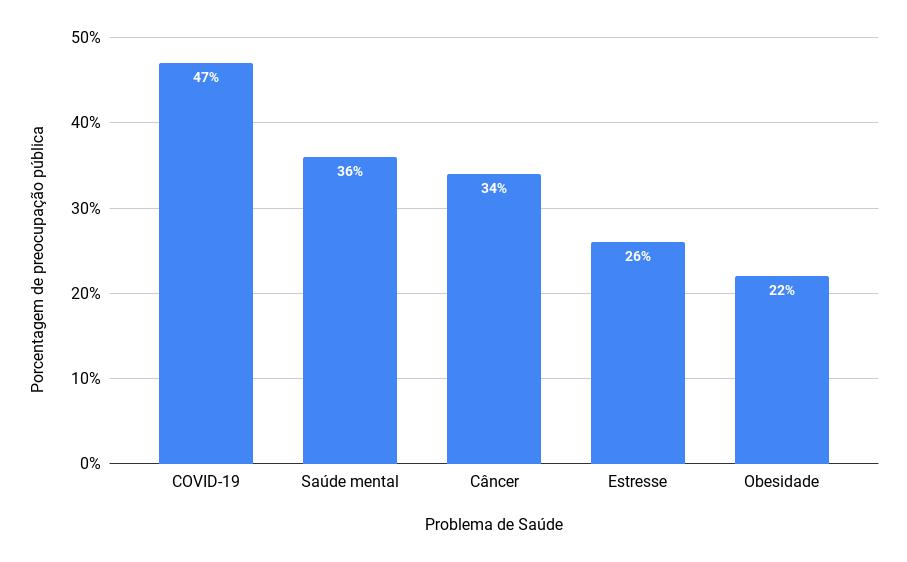
\includegraphics[width=.8\textwidth]{data/figures/interesse-publico.png}
    \fonte{\citeonline{IPSOS2022}}
\end{figure}

Nessa mesma pesquisa constata-se também que dos 34 países incluídos, o Brasil é o sétimo país que mais relata preocupação com saúde mental, onde 49\% dos brasileiros entrevistados a consideram como o problema de saúde mais enfrentado no país atualmente, estando muito acima da média global.
